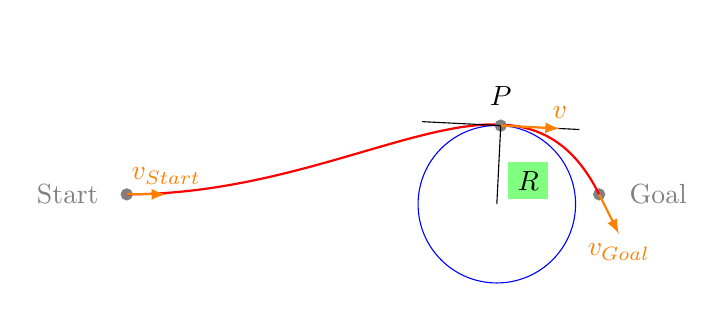
\begin{tikzpicture}
    \node (zero) at (0,0) {};
    \filldraw [gray] ([xshift=-3cm,yshift=-2cm] zero) circle (2pt) + (6,0) circle (2pt);
    \node[color=gray] at ([xshift=-3.75cm,yshift=-2cm] zero) {Start};
    \node[color=gray] at ([xshift=3.75cm,yshift=-2cm] zero) {Goal};
    
    % Trajectory
    \draw[thick,color=red]
    (-3,-2) .. controls +(3,0) and +(-1,2) .. +(6,0);

      % Point in gray
      \filldraw [gray] ([xshift=1.75cm,yshift=-1.1262cm] zero) circle (2pt);
      % Name of the point: P
      \node at ([xshift=1.75cm,yshift=-0.75cm]zero) {$P$};


        % Osculting circle
        \draw[color=blue] (1.7,-2.125) circle (1cm);
        % Drawig Ray to the plot 
        \draw (1.7,-2.125) -- (1.75,-1.1262);
        % Ray label
        \node [fill=green!50] at (2.1,-1.8262) {$R$};
        % Tangent vector to the osculting circle along the trajectory (velocity vector)
        \draw (0.7512,-1.0762) -- (2.7488,-1.1762);

    % Speed
      \draw[-latex,thick,color=orange] (1.75,-1.1262) -- (2.4991,-1.1637)
      node[above] {$v$};

    \draw[-latex,thick,color=orange] (-3,-2) -- (-2.5,-2)
    node[above]{$v_{Start}$};
    
    \draw[-latex,thick,color=orange] (3.0,-2) -- (3.25,-2.5)
    node[below]{$v_{Goal}$};
\end{tikzpicture}